\section{Modellazione dei protocolli mediante UML}

Per la modellazione di protocolli\footnote{per protocolli si intendono protocolli di sicurezza come Needham Schroeder Symmetric Key, protocolli di comunicazione come ARP e protocolli di encryption come RSA} si è deciso di utilizzare lo standard UML (Unified Modeling Language) nella versione 2.4\footnote{\url{https://www.omg.org/spec/UML/2.4/About-UML/}}, perch\'e questo tipo di modellazione utilizza una notazione semi-grafica che consente al progettista di ragionare sulla logica del protocollo che \`e pi\`u semplice rispetto al codice, senza dover porre eccessiva attenzione a come effettivamente deve essere implementato e senza dover necessariamente scrivere codice per la sua rappresentazione.\\  
Esistono 14 tipi di diagrammi nella modellazione UML, suddivisi in diagrammi strutturali e diagrammi comportamentali (o di interazione).\\ 
Tra i vari tipi di diagrammi troviamo il sequence diagram, un diagramma comportamentale, definito per la rappresentazione dettagliata delle interazioni tra gli agenti (componenti hardware o software) partecipanti al protocollo, per sua natura risulta essere il diagramma più adatto alla rappresentazione dei protocolli.\\ 
Una caratteristica di questo tipo di diagramma è che l'asse verticale rappresenta il tempo, quindi è possibile rappresentare l'ordine cronologico delle interazioni tra gli agenti partecipanti, dall'alto verso il basso.\\
In alternativa può essere utilizzato l'object diagram, un diagramma di tipo strutturale nel quale vengono rappresentate le relazioni tra i vari oggetti che compongono il sistema, nel nostro caso le relazioni e gli oggetti corrispondono rispettivamente a interazioni e agenti del sequence diagram.\\
Gli altri 12 tipi di diagramma sono stati esclusi dai possibili diagrammi utili per rappresentare protocolli perch\'e descrivono aspetti ortogonali alle interazioni descritte nel sequence diagram.\\
Nella Sezione \ref{sub:con} verrà spiegato in dettaglio perch\'e si può utilizzare indifferentemente uno tra il sequence diagram e l'object diagram.

\subsection{Confronto tra sequence diagram e object diagram}\label{sub:con}

Per la modellazione tramite lo standard UML è stato utilizzato il tool, open source, Modelio\footnote{\url{https://www.modelio.org/}} nella versione 4.1.\\
Dato il protocollo Needham Schroeder Symmetric Key descritto in \cite{NS78}:
\begin{lstlisting}[mathescape]
    1. $A \rightarrow S : A, B, N_a$
    2. $S \rightarrow A : \{N_a, K_{ab}, B, \{K_{ab}, A\}_{K_{bs}}\}_{K_{as}}$
    3. $A \rightarrow B : \{K_{ab}, A\}_{K_{bs}}$
    4. $B \rightarrow A : \{N_b\}_{K_{as}}$
    5. $A \rightarrow B : \{N_b-1\}_{K_{as}}$
\end{lstlisting}
\noindent Dove:
\begin{itemize}
    \item $X \rightarrow Y : m$ indica che il principal \texttt{X} invia un messaggio al principal \texttt{Y},
    \item $N_x$ indica il nonce generato dal principal \texttt{X},
    \item $K_{xy}$ indica la chiave condivisa tra i principal \texttt{X} e \texttt{Y},
    \item $\{\dots\}_{K_{xy}}$ indica che il pacchetto è cifrato con la chiave condivisa tra i principal \texttt{X} e \texttt{Y}.
\end{itemize}
Le figure \ref{fig:sd}-\ref{fig:od}, rappresentano il terzo messaggio del protocollo rispettivamente con un sequence ed un object diagram.\\
Più precisamente vengono rappresentate le operazioni fatte dall'agente \texttt{A} una volta ricevuta la chiave simmetrica da utilizzare con \texttt{B} dal server \texttt{S}.\\
L'agente \texttt{A} decifra con la chiave condivisa con il server \texttt{S} il pacchetto, ed inoltra all'agente \texttt{B} il pacchetto cifrato con la chiave condivisa tra \texttt{B} e \texttt{S}, contenente la chiave simmetrica tra \texttt{A} e \texttt{B}.\\

\begin{figure}[h!] 
    \centering 
        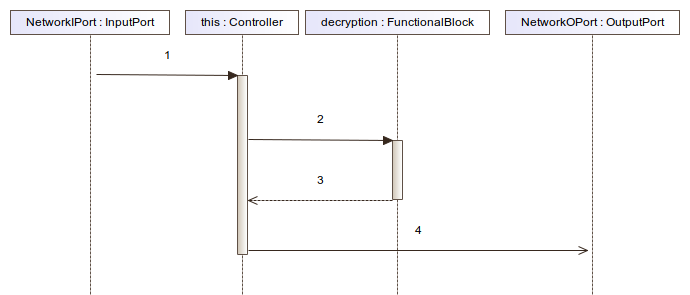
\includegraphics[width=0.8\textwidth]{../img/FirstMessage.png} 
        \caption{Sequence diagram: Inoltro pacchetto da \texttt{A} a \texttt{B}} 
        \label{fig:sd}
\end{figure}

\begin{figure}[h!]
    \centering 
    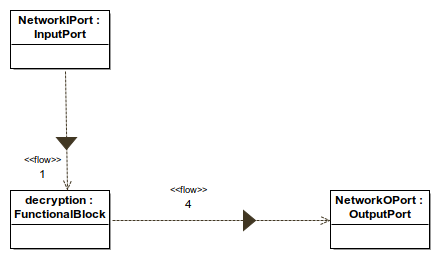
\includegraphics[scale=0.6]{../img/FirstMessage_2.png} 
    \caption{Object diagram: Inoltro pacchetto da \texttt{A} a \texttt{B}} 
    \label{fig:od}
\end{figure}

\begin{lstlisting}[frame=single, mathescape, basicstyle=\footnotesize]
1. $\{N_a, K_{ab}, B, \{K_{ab}, A\}_{K_{bs}}\}_{K_{as}}$
2. $\{N_a, K_{ab}, B, \{K_{ab}, A\}_{K_{bs}}\}_{K_{as}}$
3. $\{N_a, K_{ab}, B, \{K_{ab}, A\}_{K_{bs}}\}$
4. $\{K_{ab},A\}_{K_{bs}}$
\end{lstlisting}

\noindent Durante la fase di ingegnerizzazione di un sistema viene modellata la parte fisica, ovvero le componenti hardware che compongono il sistema, l'obiettivo è quello di unirla alla modellazione logica del funzionamento del protocollo attraverso la modellazione UML.\\
Per fare questo si è resa necessaria l'introduzione di nuovi tipi\footnote{con abuso di notazione, quando si parla di tipi di elementi, si intende la tipologia degli oggetti della classe istanziata} di elementi, che non appartengono ai tipi degli elementi standard dei diagrammi UML.\\
\begin{figure}[h!]
    \centering
    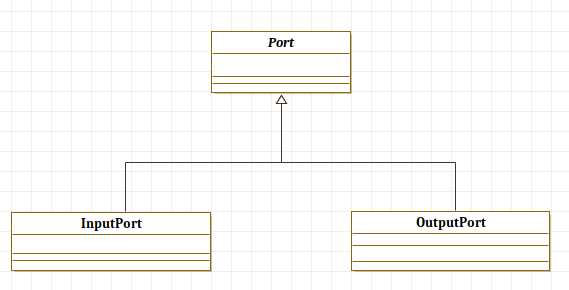
\includegraphics[width=0.6\textwidth]{../img/cdport.png} 
    \caption{Class diagram Port}
    \label{fig:cdport}
\end{figure}

\noindent Come vediamo in Figura \ref{fig:cdport} sono stati definiti i tipi InputPort e OutPort, specializzazioni del tipo Port.\\
Questi tipi di oggetti vengono utilizzati nelle due tipologie di diagramma come unico punto di contatto tra i modelli del software e dell'hardware, infatti sono le componenti utilizzate dai protocolli per ricevere o inoltrare messaggi.\\
Inoltre, guardando le lifelines in Figura \ref{fig:sd} si può notare anche il Controller, il quale è il dispositivo proprietario delle porte.\\
Anche per la modellazione logica del funzionamento del protocollo si è resa necessaria l'introduzione di nuovi tipi.\\
\begin{figure}[h!]
    \centering
    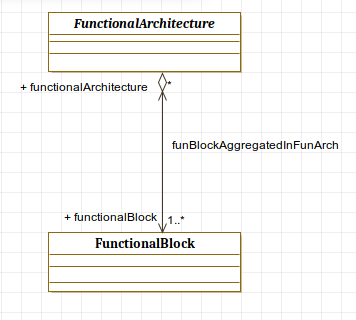
\includegraphics[width=0.5\textwidth]{../img/cdfun.png} 
    \caption{Class diagram Function}
    \label{fig:cdfun}
\end{figure}

\noindent Gli elementi di tipo FunctionalBlock vengono utilizzati per la codifica di un'operazione che non può essere dettagliata maggiormente (oppure non è necessario farlo considerando l'obiettivo della verifica di questo modello) che, presi degli input, restituisce un output.\\
Nel caso in cui si voglia rappresentare un insieme di operazioni si utilizzano gli elementi di tipo FunctionalArchitecture, questi vengono utilizzati come ``segnaposto'' per l'insieme di operazioni che verrà descritto in un altro diagramma dello stesso tipo di quello utilizzato, avente come nome lo stesso dato all'elemento di tipo FunctionalArchitecture.\\
Infatti come vediamo in Figura \ref{fig:cdfun} una FunctionalArchitecture può essere composta da uno o più elementi di tipo FunctionalBlock.\\
In entrambi i diagrammi le InformationFlow rappresentano gli input e gli output dei vari elementi, nelle etichette vengono descritti i parametri passati, per convenzione se i parametri si trovano tra \{ \} significa che l'input o l'output di un oggetto è un pacchetto.\\
Modelio consente di esportare i modelli UML in file .xmi (XML Metadata Interchange), uno standard basato sulla struttura XML che ne consente lo scambio tra applicazioni.\\
Nel file .xmi, strutturato come un xml, troviamo i tag per l'identificazione tramite codice univoco (id) degli elementi (lifelines, oggetti, InformationFlow) e i tag per descrivere le proprietà dei vari elementi (tipo, nome, descrizione). Tra le proprietà degli elementi di tipo InformationFlow sono presenti i tag per identificare tramite id l'elemento sorgente e l'elemento destinazione delle informazioni. Analizzando il file .xmi estratto da un protocollo modellato tramite sequence diagram (Listing \ref{fig:sdxmi}) o da un protocollo modellato tramite object diagram (Listing \ref{fig:odxmi}), possiamo vedere come l'estrazione delle lifelines del sequence diagram corrisponde all'estrazione degli oggetti dell'object diagram (righe 7-12) e l'estrazione delle information flow viene rappresentata nello stesso modo (righe 14-20).\\
\begin{minipage}{0.48\textwidth}
      \centering
      \lstinputlisting[label={fig:sdxmi},caption={Estratto di XMI da sequence diagram},mathescape,numbers=left, language=XMI, breaklines= true, frame=single]{../xmi/ns_estratto_seq_2.xmi}
    \end{minipage}\hfill
    \begin{minipage}{0.48\textwidth}
      \centering
      \lstinputlisting[label={fig:odxmi},caption={Estratto di XMI da object diagram},mathescape, language=XMI, breaklines= true, frame=single]{../xmi/ns_estratto_ob_2.xmi} 
\end{minipage}
\newpage

\noindent Questo ci consente di affermare che utilizzando uno a scelta tra i due diagrammi è possibile modellare un protocollo senza la perdita di alcuna informazione.\\
Il file .xmi può essere utilizzato come input di un software in grado di navigarne la struttura e restituire in output dei file pronti per essere utilizzati dai tool di verifica formale e automatica dei protocolli, ad esempio nella Sezione \ref{sez:tc} viene presentato un software, da me sviluppato, in grado di restituire come output un file scritto nel linguaggio specifico per essere utilizzato come input dal tool di verifica automatica VerifPal.

\begin{figure}[h!]
    \centering
    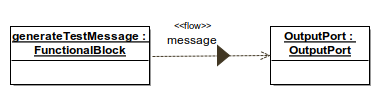
\includegraphics[scale=0.6]{../xmi/ex.png} 
    \caption{Esempio di modellazione con object diagram}
    \label{fig:exUML}
\end{figure}

\begin{figure} [h!]
    \centering
    \lstinputlisting[language=XMI, breaklines= true, frame=single]{../xmi/ex.xmi}
    \caption{Esempio di estrazione di un file .xmi}
\end{figure}

\clearpage
